\subsection{Data}

\begin{figure}[h!]
\centering
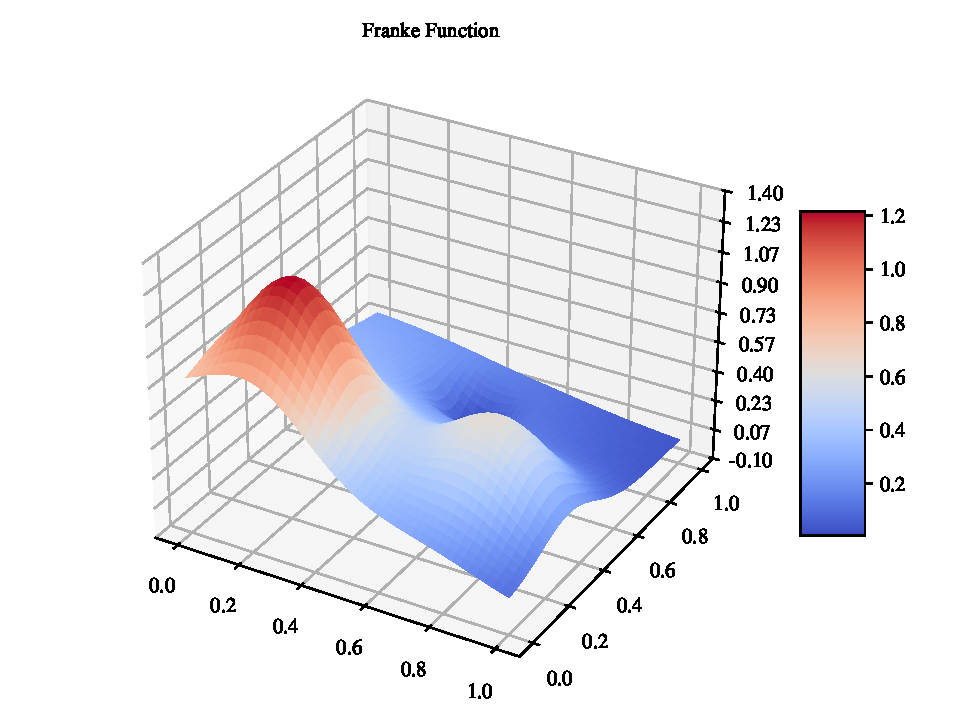
\includegraphics[width=1\linewidth]{project_1_alt/figures/data/franke_func.pdf}
\caption{Franke function for x,y $\in [0,1]$}
\label{franke}
\end{figure}
\subsubsection{Franke Function}
We first implement our methods on a synthetic data-set based on the Franke Function \citep[p. 13]{frank}. Originally proposed by Richard Franke in 1979 is a much used function for testing linear regression and interpolation problems.
The Franke function is defined as:
\begin{align}
    f(x, y) = &\frac{3}{4} \exp\left( -\frac{(9x - 2)^2}{4} - \frac{(9y - 2)^2}{4} \right) \nonumber \\
    + &\frac{3}{4} \exp\left( -\frac{(9x + 1)^2}{49} - \frac{(9y + 1)^2}{10} \right) \nonumber \\
    + &\frac{1}{2} \exp\left( -\frac{(9x - 7)^2}{4} - \frac{(9y - 3)^2}{4} \right) \nonumber \\
    - &\frac{1}{5} \exp\left( -(9x - 4)^2 - (9y - 7)^2 \right)
\end{align}




\begin{figure}[h!]
\centering
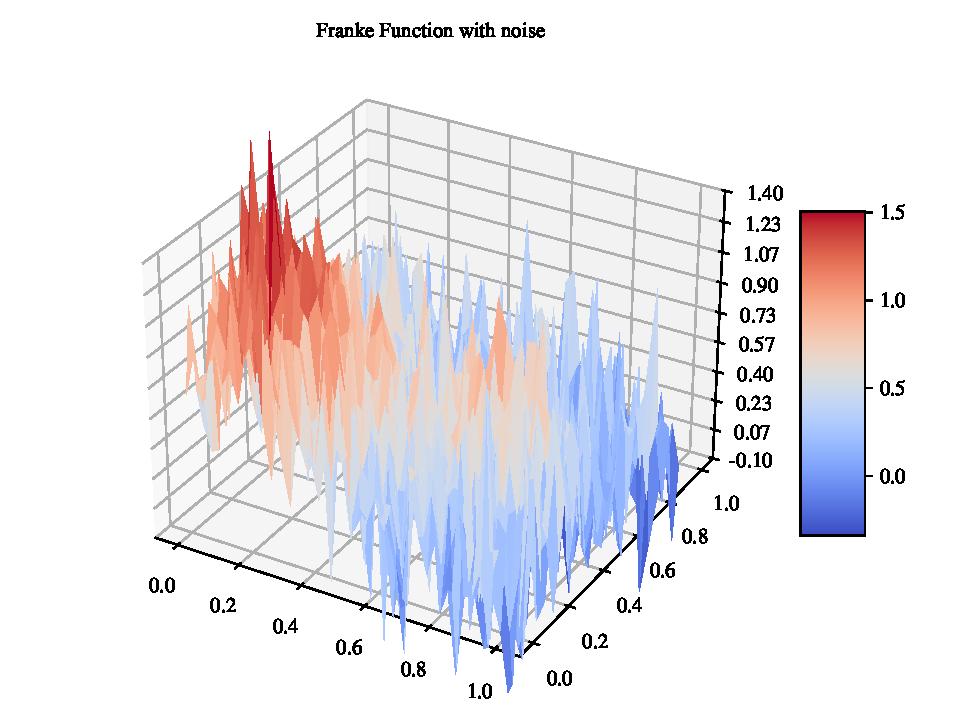
\includegraphics[width=1\linewidth]{project_1_alt/figures/data/franke_func_noise.pdf}
\caption{Franke function for x,y $\in [0,1]$ with noise \mia{...}}
\label{franke_noise}
\end{figure}


\subsubsection{Terrain data}

\begin{figure}
    \centering
    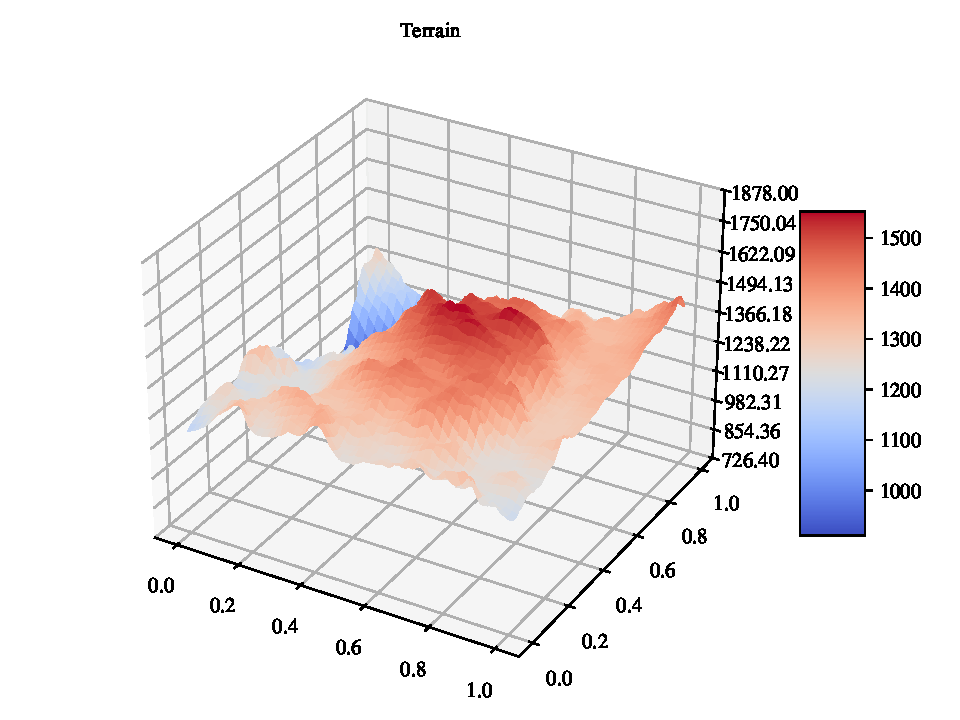
\includegraphics[width=1\linewidth]{project_1_alt/figures/data/terrain_data.pdf}
    \caption{Terrain data}
    \label{data:terrain}
\end{figure}

\mia{må skrive noe her}

\subsection{Hyperparameter selection}
All the linear model types in this project (OLS, Ridge and Lasso) have hyperparameters which results in different models. 
These hyperparameters are the model complexity (i.e. the maximum degree of $x$ and $y$ in the resulting expression) and the weight parameter for the regularization for Ridge and Lasso regression ($\lambda$). 
Optimizing the Ordinary Least Square model is simple, as we only need to test it on different model-complexity. 
We run a set of bootstrap samples for each degree complexity, and choose the model with the lowest MSE.

For Ridge and Lasso however, we require selecting two parameters simultaneously. As different model-complexities might obtain the best MSE at different values for $\lambda$, it does not suffice to lock one and test the other only for that value. 
We use grid search, a standard technique for tuning multiple hyper parameters. \citep[p. 302]{grid_search} 
Grid search is an exhaustive search over a selection of values for each parameter. 
We perform two layers of grid search on each type of model and set of data. 
In the first layer we test model-complexities ranging from 1 to 11, and lambdas from $1*10^{-5}$ up to $9$ (with increasing step size according to order of magnitude). 
We use 200 bootstrap samples, and pick the values for complexity $d$ and $\lambda$ resulting in the lowest MSE. 
In the second layer, we use only the complexities $d-1,\ d,\ d+1$, and 40 different $\lambda$-values ranging from $(4/5)\lambda$ to $(6/5)\lambda$. 
We do this in order to fine tune our selections of hyper-parameters.
\gaute{}